\documentclass{article}
% packages
\usepackage {lmodern}
\usepackage [T1]{fontenc}
\usepackage {amsmath}
\usepackage {amssymb}
\usepackage {amsfonts}
\usepackage {graphicx}
\usepackage {fullpage}
\usepackage {gensymb}
\usepackage {caption}
\usepackage {subcaption}
\usepackage {array}
\newcolumntype{L}{>{\centering\arraybackslash}m{3cm}}
%\usepackage{nopageno}
\usepackage {cite}
\usepackage {setspace}
\usepackage [version=4]{mhchem}
\usepackage {pdfpages}
\usepackage[ampersand]{easylist}
\usepackage {fancyvrb}
\usepackage {listings}
\usepackage {color}

\definecolor{dkgreen}{rgb}{0,0.6,0}
\definecolor{gray}{rgb}{0.5,0.5,0.5}
\definecolor{mauve}{rgb}{0.58,0,0.82}

\lstset{frame=tb,
	language=C,
	aboveskip=3mm,
	belowskip=3mm,
	showstringspaces=false,
	columns=flexible,
	basicstyle={\small\ttfamily},
	numbers=none,
	numberstyle=\tiny\color{gray},
	keywordstyle=\color{blue},
	commentstyle=\color{dkgreen},
	stringstyle=\color{mauve},
	breaklines=true,
	breakatwhitespace=true,
	tabsize=3
}

\usepackage{titling}
\newcommand{\subtitle}[1]{%
    \posttitle{%
        \par\end{center}
        \begin{center}\LARGE#1\end{center}
        \vskip0.5em}%
}

\graphicspath {{images/}}

\begin{document}
\title{An Investigation on the Efficiency of \\ Multiple Sequence Alignment Tools}
\subtitle{Mid-Project Review}
\author {Justin Chao - juchao \\
		Chase Meyer - cmeyer3 \\
		Bria Lacour - lacour}
\maketitle

\section*{Project Goal}
We will be developing a Multiple Sequence Alignment (MSA) program that uses a
Markov Chain and a local alignment algorithm to optimize global alignments of
protein sequences.

The Needleman-Wunsch algorithm will be used to calculate alignments using the
BLOSUM 62 matrix as a scoring reference.

A comparison of run-times and accuracy will then be conducted
between our developed MSA tool, BLAST, and MAFFT on a series of test sequences. 

\section*{Background}
A MSA tool can be used by computational biologists to track evolutionary
relationships, predict structures, track mutations, etc. MSA tools come in a
variety of forms and are tailored to address specific biological problems.
These sequences are usually protein, DNA, or RNA, which can affect the methods
of analysis in different ways.  

The efficiency of these tools can affect scientific analyses, such as
identifying significant patterns in protein families or assessing conservation
of different genetic characteristics across species. 
The Needleman-Wunsch algorithm is used for global alignment purposes while the
Smith-Waterman algorithm is used for aligning sub-sequences. 

\begin{center}
    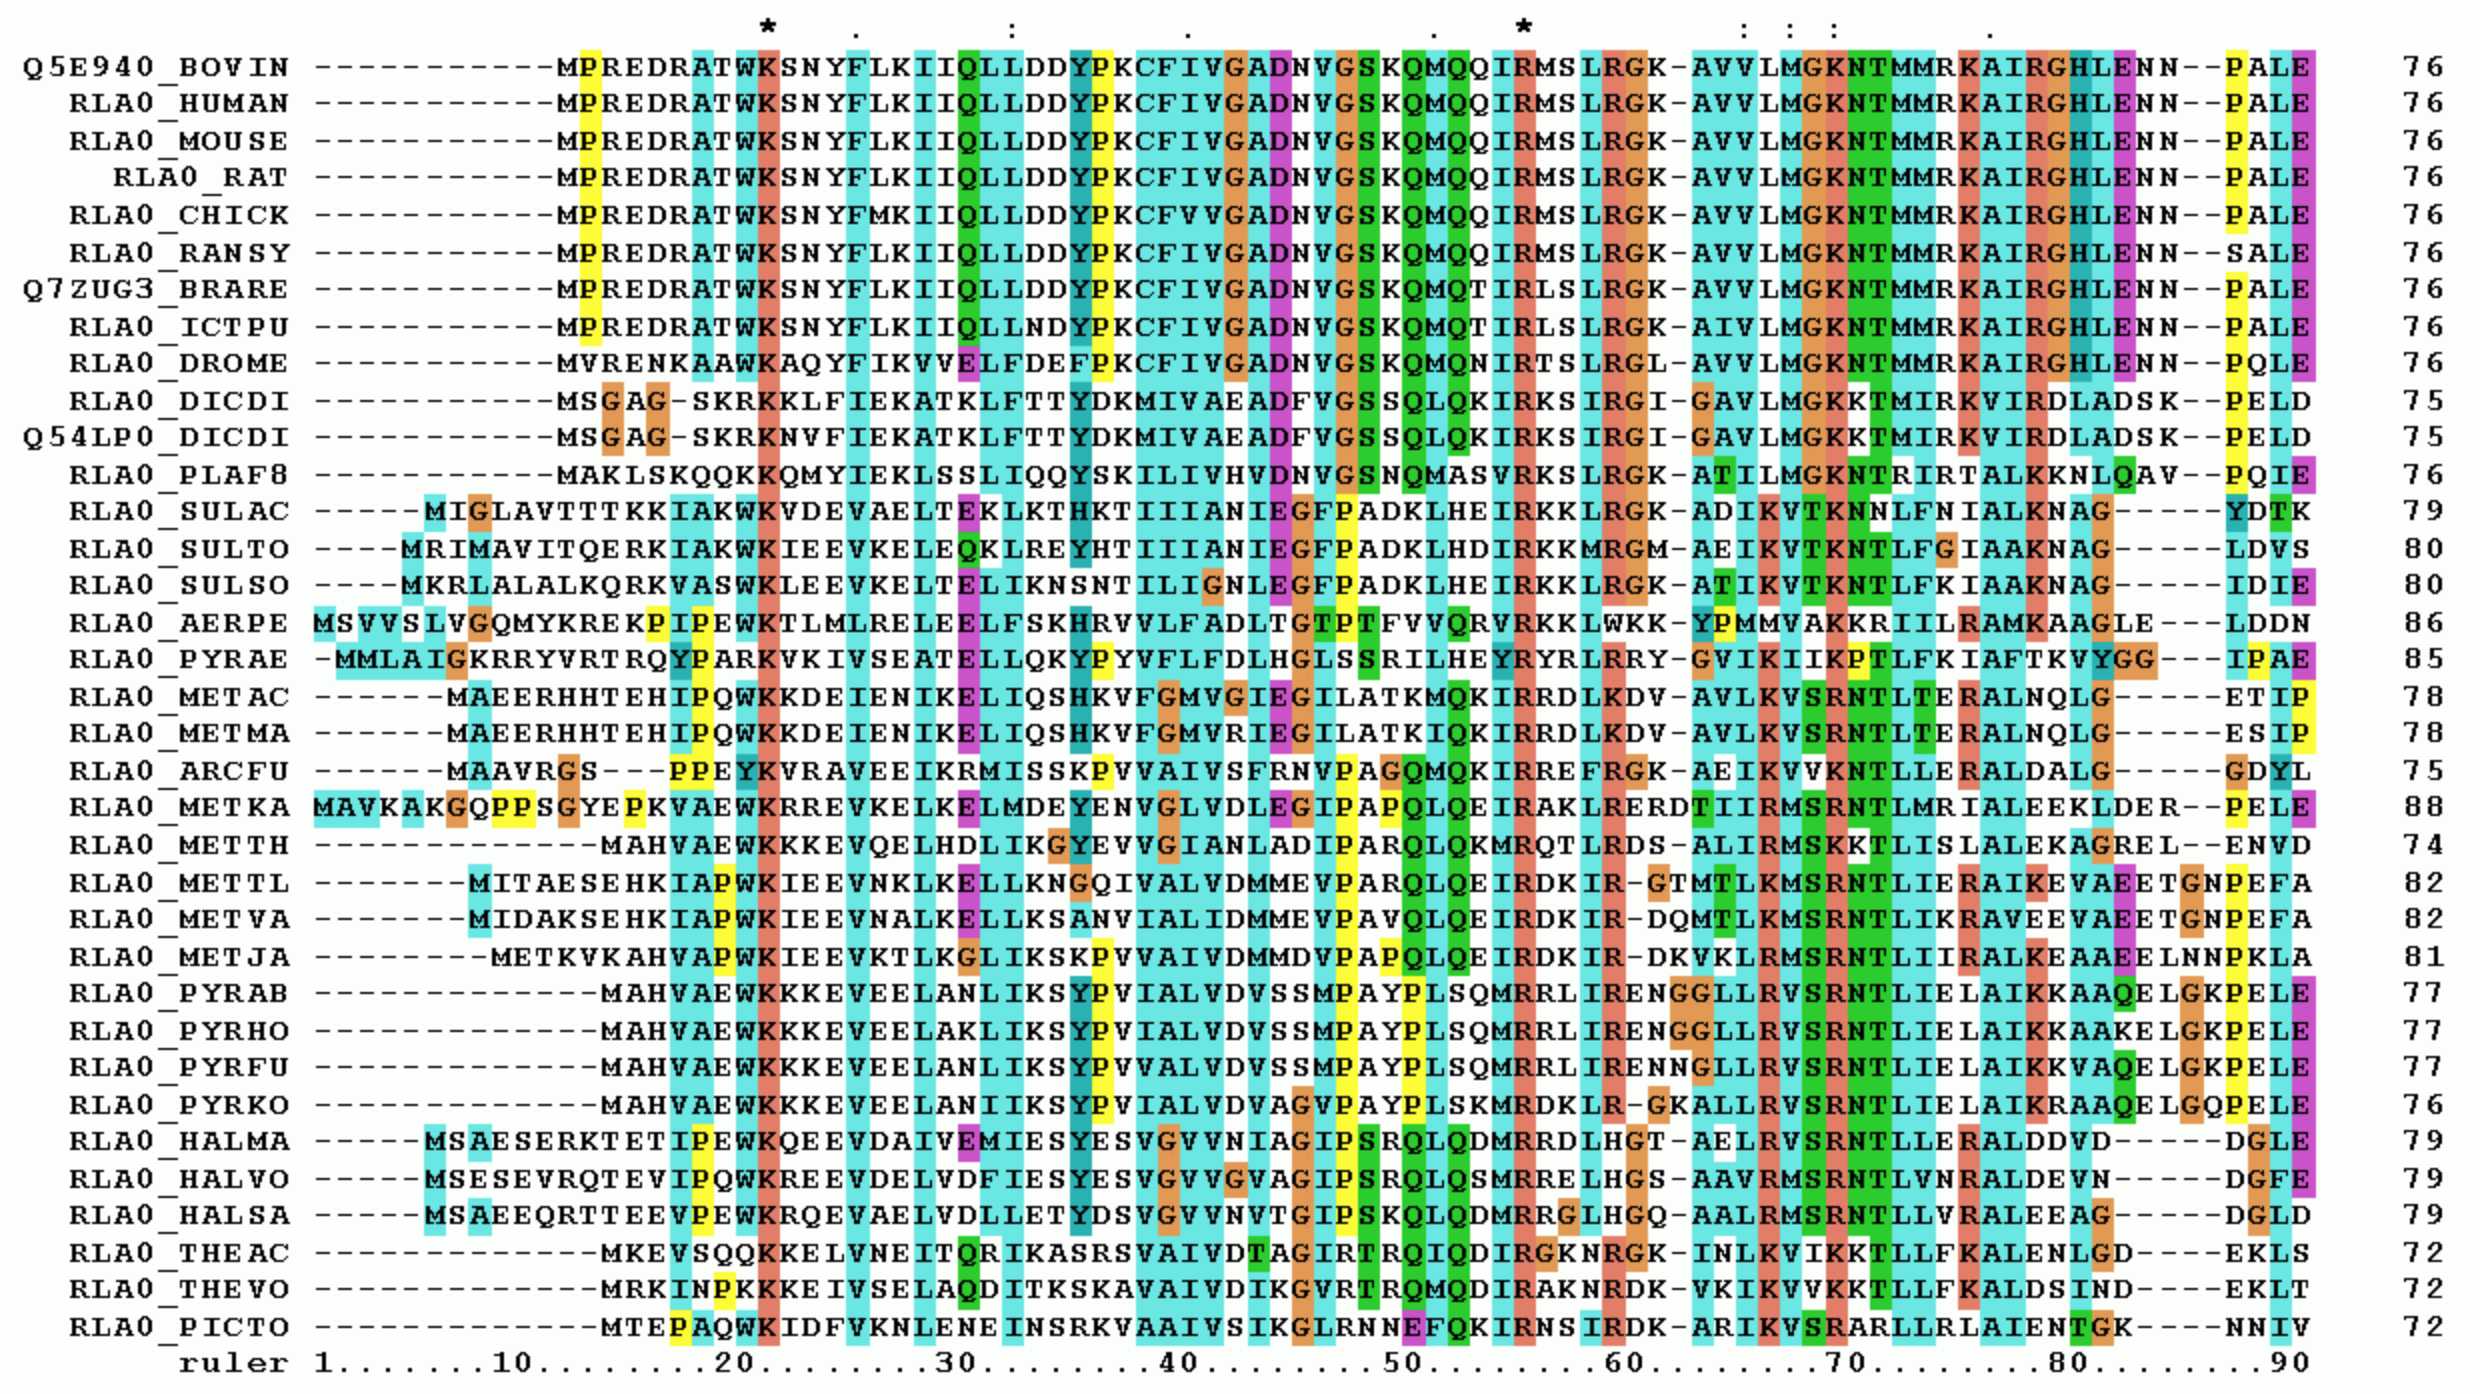
\includegraphics[scale=0.4]{multiple_alignment}
    \captionof{figure}{Representation of a protein multiple sequence alignment
    produced with ClustalW. The sequences are instances of the acidic ribosomal
    protein P0 homolog (L10E) encoded by the Rplp0 gene from multiple organisms.
    Only the first 90 positions of the alignment are displayed. The colors represent the
    amino acid conservation according to the properties and distribution of
    amino acid frequencies in each column. Note the two completely conserved
    residues arginine (R) and lysine (K) marked with an asterisk at the top of
    the alignment. \cite{multiple_alignment}}
\end{center}

\section*{Progress of Goals}
\begin{itemize}
    \item [$\boxtimes$] Code Needleman-Wunsch Algorithm.
    \item [$\boxtimes$] Code Smith-Waterman Algorithm.
    \item [$\boxtimes$] Find sample sequences for testing via NCBI.
    \item [$\square$] Parallelize algorithms.
    \item [$\square$] Calculate global alignment via Needleman-Wunsch.
    \item [$\square$] Calculate local alignments via Smith-Waterman.
    \item [$\square$] Use Markov chain to determine best local alignments.
    \item [$\square$] Align sequences using MAFFT, MUSCLE, Clustal Omega, and
        PRANK for comparison.
    \item [$\square$] Compare accuracy and run-time efficiency of
        results.
    \item [$\square$] Create visual diagram comparing alignment results of
        various MSA algorithms
\end{itemize}


\newpage
\section*{Algorithms}
The following are algorithms that will be used in the creation of our MSA tool.
\cite{wilke} \cite{fft}

\subsection*{Needleman-Wunsch Algorithm}
\begin{align*}
    M(0, j) = j \times p  \hspace{1cm}&\text{for first row, where p is the gap
    penalty} \\
    M(i, 0) = i \times p  \hspace{1cm}&\text{for first column}
\end{align*}

\begin{equation*}
    M(0, j) = max \begin{cases}
        M(i-1, j) + p & \text{top} \\
        M(i, j-1) + p & \text{left} \\
        M(i-1, j-1) + s(a_j , b_i) & \text{diagonal}
  \end{cases}
\end{equation*}

Where $s(a_j , b_i)$ = match/mismatch score for sites j and i in sequences a and
b. \cite{columbia}

\subsection*{Smith-Waterman Algorithm}
\begin{align*}
    M(0, j) = j \times p  \hspace{1cm}&\text{for first row} \\
    M(i, 0) = i \times p  \hspace{1cm}&\text{for first column}
\end{align*}

\begin{equation*}
    M(0, j) = max \begin{cases}
        0 \\
        M(i-1, j) + p & \text{top} \\
        M(i, j-1) + p & \text{left} \\
        M(i-1, j-1) + s(a_j , b_i) & \text{diagonal}
  \end{cases}
\end{equation*}

Where $s(a_j , b_i)$ = match/mismatch score for sites j and i in sequences a and
b. \cite{columbia}

\vspace{2cm}
\begin{center}
    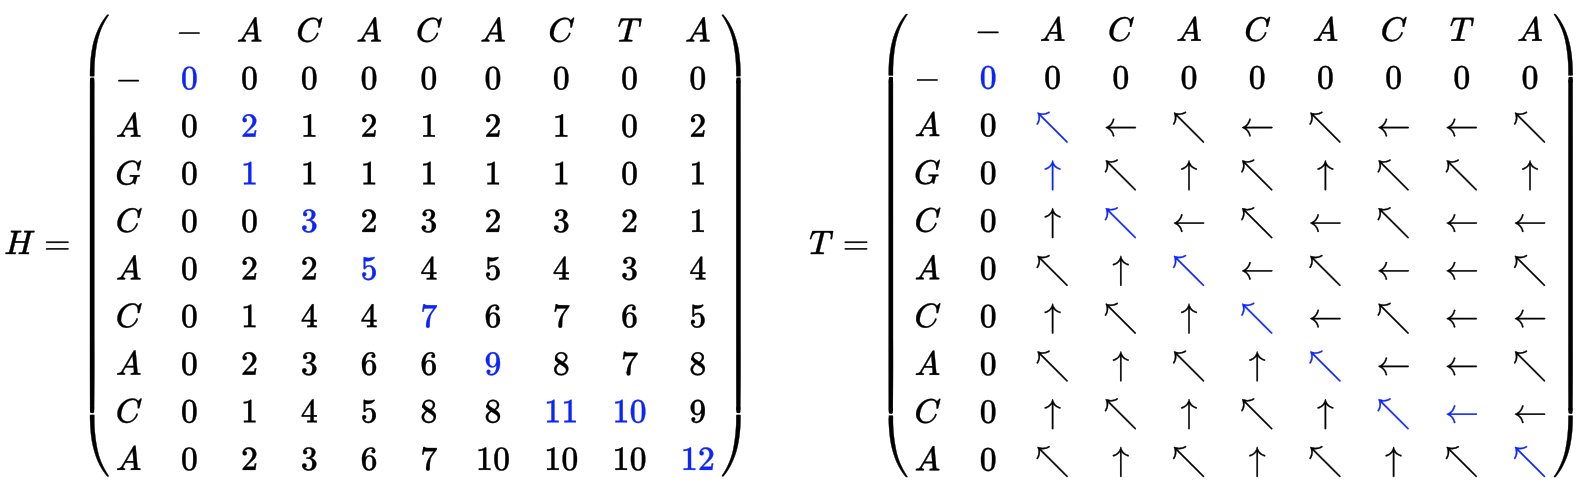
\includegraphics[scale=0.5]{sw.png}
    \captionof{figure}{Visual representation of Smith-Waterman algorithm.
    \cite{sw}}
\end{center}

\newpage
\section*{Code Examples}
\subsubsection*{Needleman-Wunsch Algorithm}
\begin{lstlisting}
# nw_example.c

#include <stdlib.h>
#include <stdio.h>
#include <string.h>

#include "needleman_wunsch.h"

void align(char* seq_a, char* seq_b) {
  	// Variables to store alignment result
  	nw_aligner_t *nw = needleman_wunsch_new();
  	alignment_t *result = alignment_create(256);
		
  	// Decide on scoring
  	int match = 1;
  	int mismatch = -2;
  	int gap_open = -4;
  	int gap_extend = -1;
 		 
  	// Don't penalise gaps at the start
  	// ACGATTT
  	// ----TTT would score +3 (when match=+1)
  	char no_start_gap_penalty = 1;
 		 
  	// ..or gaps at the end e.g.
  	// ACGATTT
  	// ACGA--- would score +4 (when match=+1)
  	char no_end_gap_penalty = 1;
		
  	char no_gaps_in_a = 0, no_gaps_in_b = 0;
  	char no_mismatches = 0;
		
  	// Compare character case-sensitively (usually set to 0 for DNA etc)
  	char case_sensitive = 0;
		
  	scoring_t scoring;
  	scoring_init(&scoring, match, mismatch, gap_open, gap_extend,
               no_start_gap_penalty, no_end_gap_penalty,
               no_gaps_in_a, no_gaps_in_b, no_mismatches, case_sensitive);
	
  	// Add some special cases
  	// x -> y means x in seq1 changing to y in seq2
  	scoring_add_mutation(&scoring, 'a', 'c', -2); // a -> c give substitution score -2
  	scoring_add_mutation(&scoring, 'c', 'a', -1); // c -> a give substitution score -1
		
  	// We could also prohibit the aligning of characters not given as special cases
  	// scoring.use_match_mismatch = 0;
		
  	needleman_wunsch_align(seq_a, seq_b, &scoring, nw, result);
		
  	printf("seqA: %s\n", result->result_a);
  	printf("seqB: %s\n", result->result_b);
  	printf("alignment score: %i\n", result->score);
		
	// Free memory for storing alignment results
	needleman_wunsch_free(nw);
	alignment_free(result);
}

int main(int argc, char* argv[]) {
	if(argc != 3) {
		printf("usage: ./nw_example <seq1> <seq2>\n");
		exit(EXIT_FAILURE);
  	}

  	align(argv[1], argv[2]);
  	exit(EXIT_SUCCESS);
}
\end{lstlisting}

\subsubsection*{Smith-Waterman Algorithm}
\begin{lstlisting}
# sw_example.c

#include <stdlib.h>
#include <stdio.h>
#include <string.h>

#include "smith_waterman.h"

void align(char* seq_a, char* seq_b)
{
	// Variables to store alignment result
	sw_aligner_t *sw = smith_waterman_new();
	alignment_t *result = alignment_create(256);
	
	// Decide on scoring
	int match = 1;
	int mismatch = -2;
	int gap_open = -4;
	int gap_extend = -1;
 	 
	// Don't penalise gaps at the start
	// ACGATTT
	// ----TTT would score +3 (when match=+1)
	char no_start_gap_penalty = 1;
 	 
	// ..or gaps at the end e.g.
	// ACGATTT
	// ACGA--- would score +4 (when match=+1)
	char no_end_gap_penalty = 1;
	
	char no_gaps_in_a = 0, no_gaps_in_b = 0;
	char no_mismatches = 0;

	// Compare character case-sensitively (usually set to 0 for DNA etc)
	char case_sensitive = 0;
		
  	scoring_t scoring;
  	scoring_init(&scoring, match, mismatch, gap_open, gap_extend,
               no_start_gap_penalty, no_end_gap_penalty,
               no_gaps_in_a, no_gaps_in_b, no_mismatches, case_sensitive);
	
  	// Add some special cases
  	// x -> y means x in seq1 changing to y in seq2
  	scoring_add_mutation(&scoring, 'a', 'c', -2); // a -> c give substitution score -2
  	scoring_add_mutation(&scoring, 'c', 'a', -1); // c -> a give substitution score -1
		
  	// We could also prohibit the aligning of characters not given as special cases
  	// scoring.use_match_mismatch = 0;
		
  	smith_waterman_align(seq_a, seq_b, &scoring, sw);
		
  	while(smith_waterman_fetch(sw, result))
  	{
    	printf("seqA: %s [start:%zu]\n", result->result_a, result->pos_a);
    	printf("seqB: %s [start:%zu]\n", result->result_b, result->pos_b);
    	printf("alignment score: %i\n\n", result->score);
  	}
	
  	// Free memory for storing alignment results
  	smith_waterman_free(sw);
  	alignment_free(result);
}

int main(int argc, char* argv[])
{
	if(argc != 3)
	{
    	printf("usage: ./sw_example <seq1> <seq2>\n");
    	exit(EXIT_FAILURE);
  	}
		
  	align(argv[1], argv[2]);
  	exit(EXIT_SUCCESS);
}
\end{lstlisting}
\cite{code}

\newpage
\section*{Appendix}
\begin{center}
    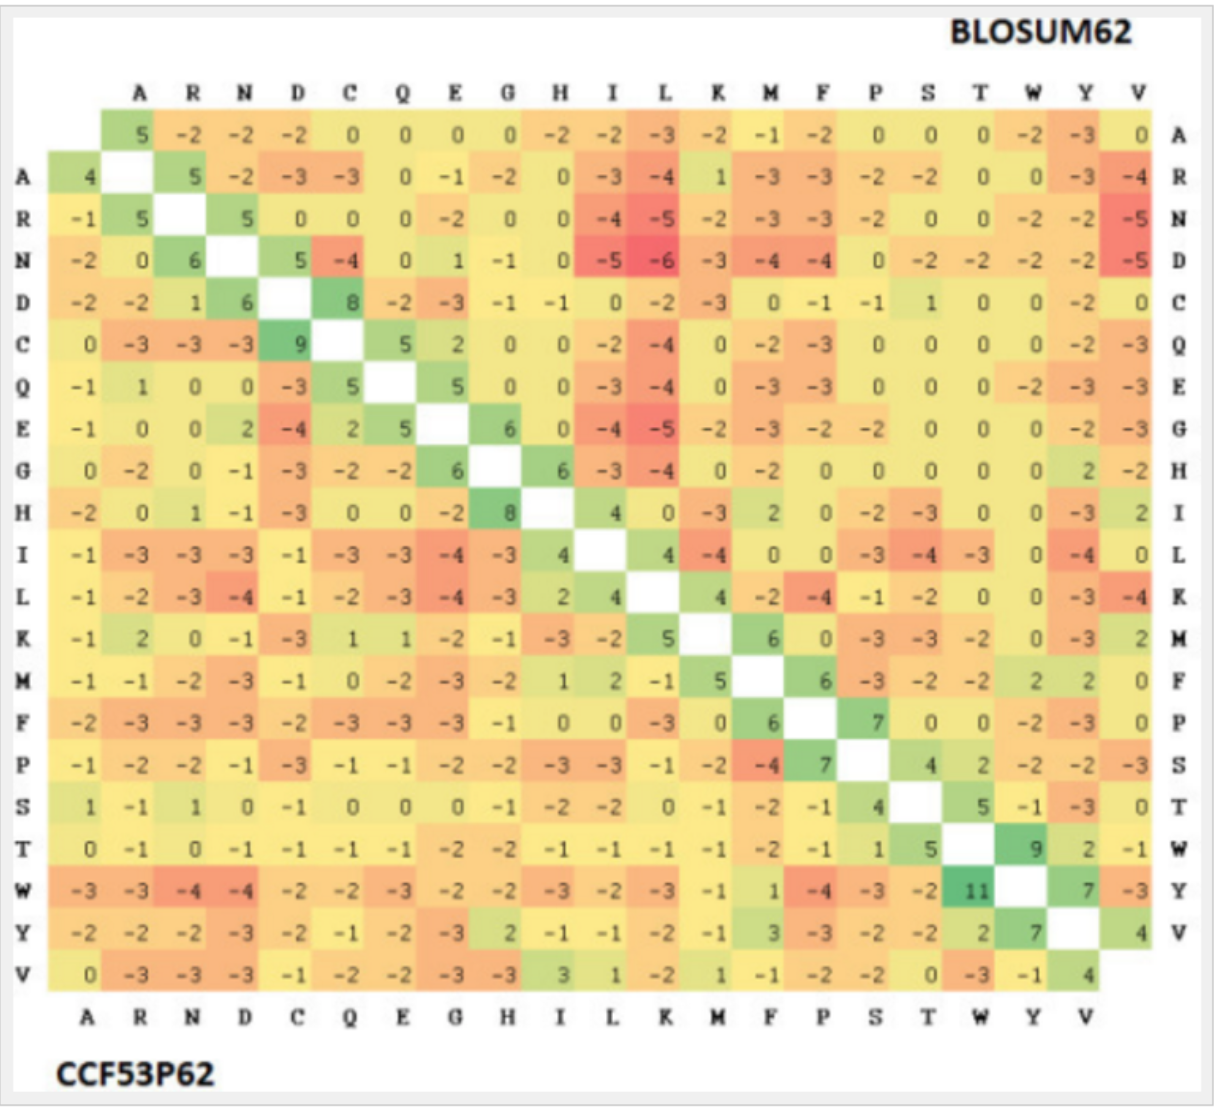
\includegraphics[scale=0.6]{BLOSUM}
    \captionof{figure}{Comparison of BLOSUM62 and CCF53\_62 matrices. The
    BLOSUM62 matrix is given on the upper right, while CCF53 is given on the
    lower left. Positive substitution scores are colored green, while negative
    scores are red. Deeper colors represent more positive/negative
    scores.\cite{blosum}}

    \vspace {1.5cm}
    \resizebox{0.5\textwidth}{!}{\begin{tabular}{c|c|c}
        \textbf{MSA tool} & \textbf{Speed} & \textbf{Accuracy} \\ 
        \hline
        MAFFT & very fast & medium-high \\
        MUSCLE & very fast & medium \\
        Clustal Omega & medium & medium-low \\
        PRANK & very slow & very high\\
    \end{tabular}}
    \captionof{table}{Comparison of known MSA tools. Actual sequence alignment
    times and accuracies can vary depending on sequence size and scoring
    parameters.}
\end{center}



\newpage
\bibliographystyle{unsrt}
\bibliography{mid_review.bib}

\end{document}
